\newpage
\begin{center}
  \textbf{\large ПРИЛОЖЕНИЕ А}
\end{center}
\refstepcounter{chapter}
\addcontentsline{toc}{chapter}{ПРИЛОЖЕНИЕ А}

 \begin{figure}[!ht]
        \centering
        \includegraphics[width=\textwidth]{FuncBlocks.jpg}
        \caption{Функциональная схема проектируемого устройства}
        \label{FuncBlocks}
    \end{figure}



%   \newpage
%   \afterpage{% Начинаем новую страницу после текущей
%     % Устанавливаем параметры страницы A3
%     \newgeometry{a3paper, landscape, margin=15mm}
    
%     % Вставляем PDF-файл
%     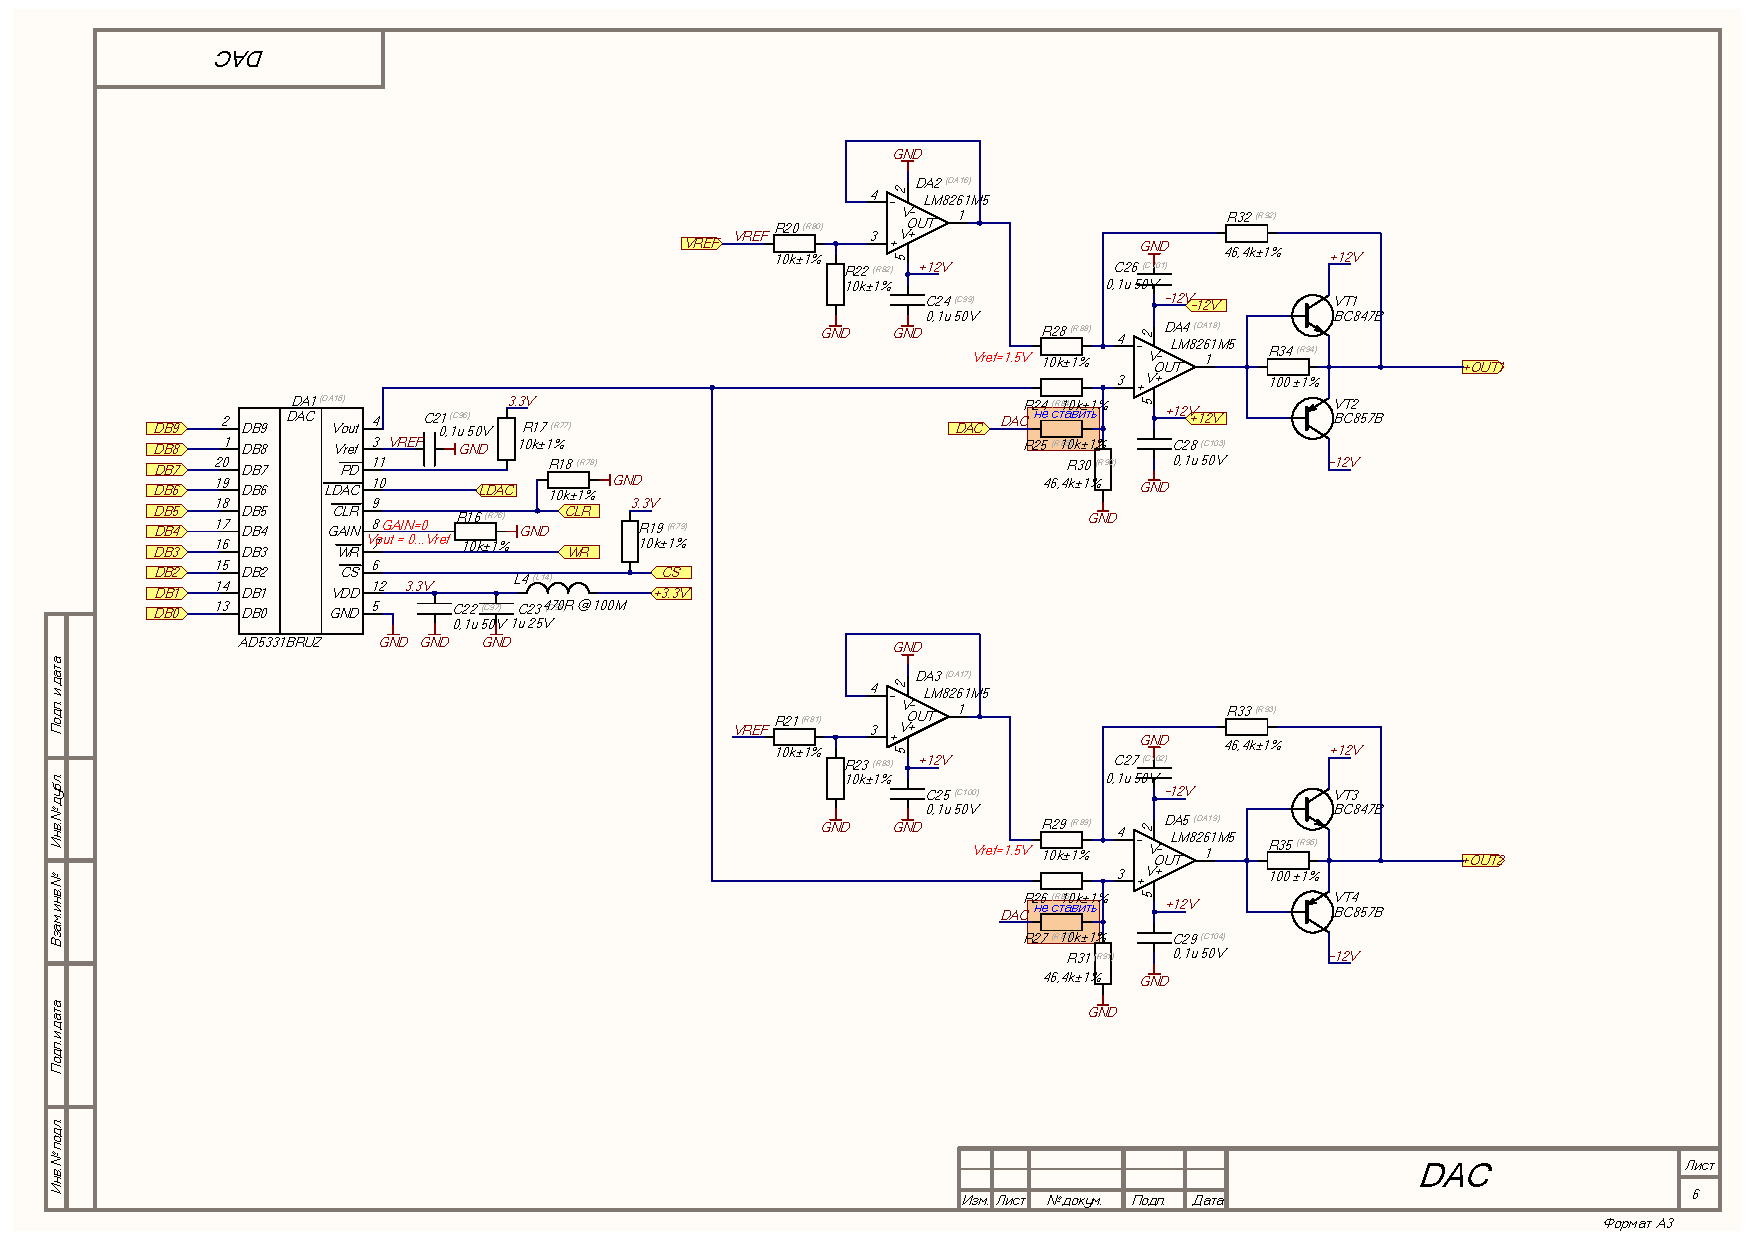
\includepdf[pages=1, 
%         scale=0.95, % Масштабирование (подберите под ваш документ)
%         pagecommand={\thispagestyle{empty}} % Отключаем колонтитулы
%     ]{DAC.pdf} % Имя вашего PDF-файла

%     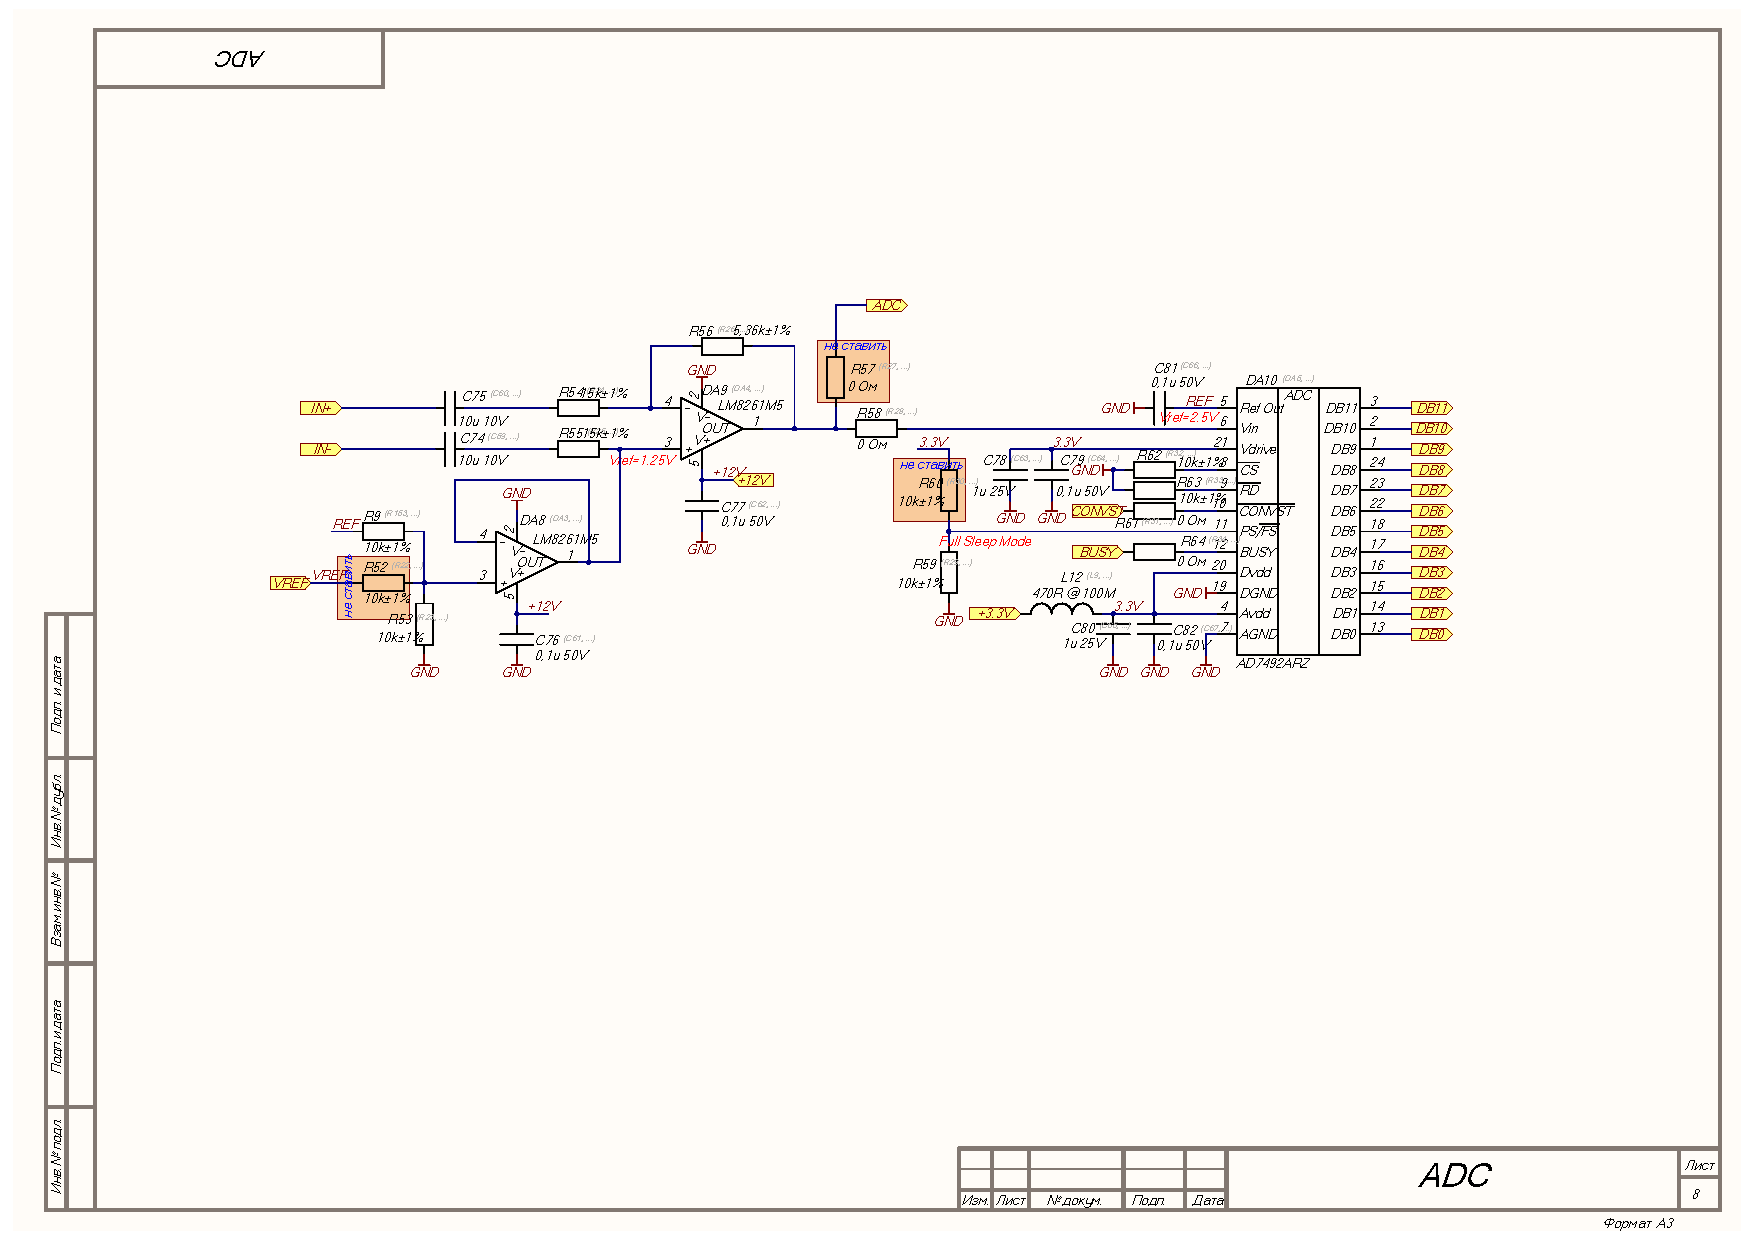
\includepdf[pages=1, 
%         scale=0.95, % Масштабирование (подберите под ваш документ)
%         pagecommand={\thispagestyle{empty}} % Отключаем колонтитулы
%     ]{ADC.pdf} % Имя вашего PDF-файла
    
%     % Возвращаем настройки A4 для последующих страниц
%     \restoregeometry
% }


\clearpage
% \newgeometry{a3paper, vertical, margin=15mm}
% \begin{figure}[h!]
%     \centering
%     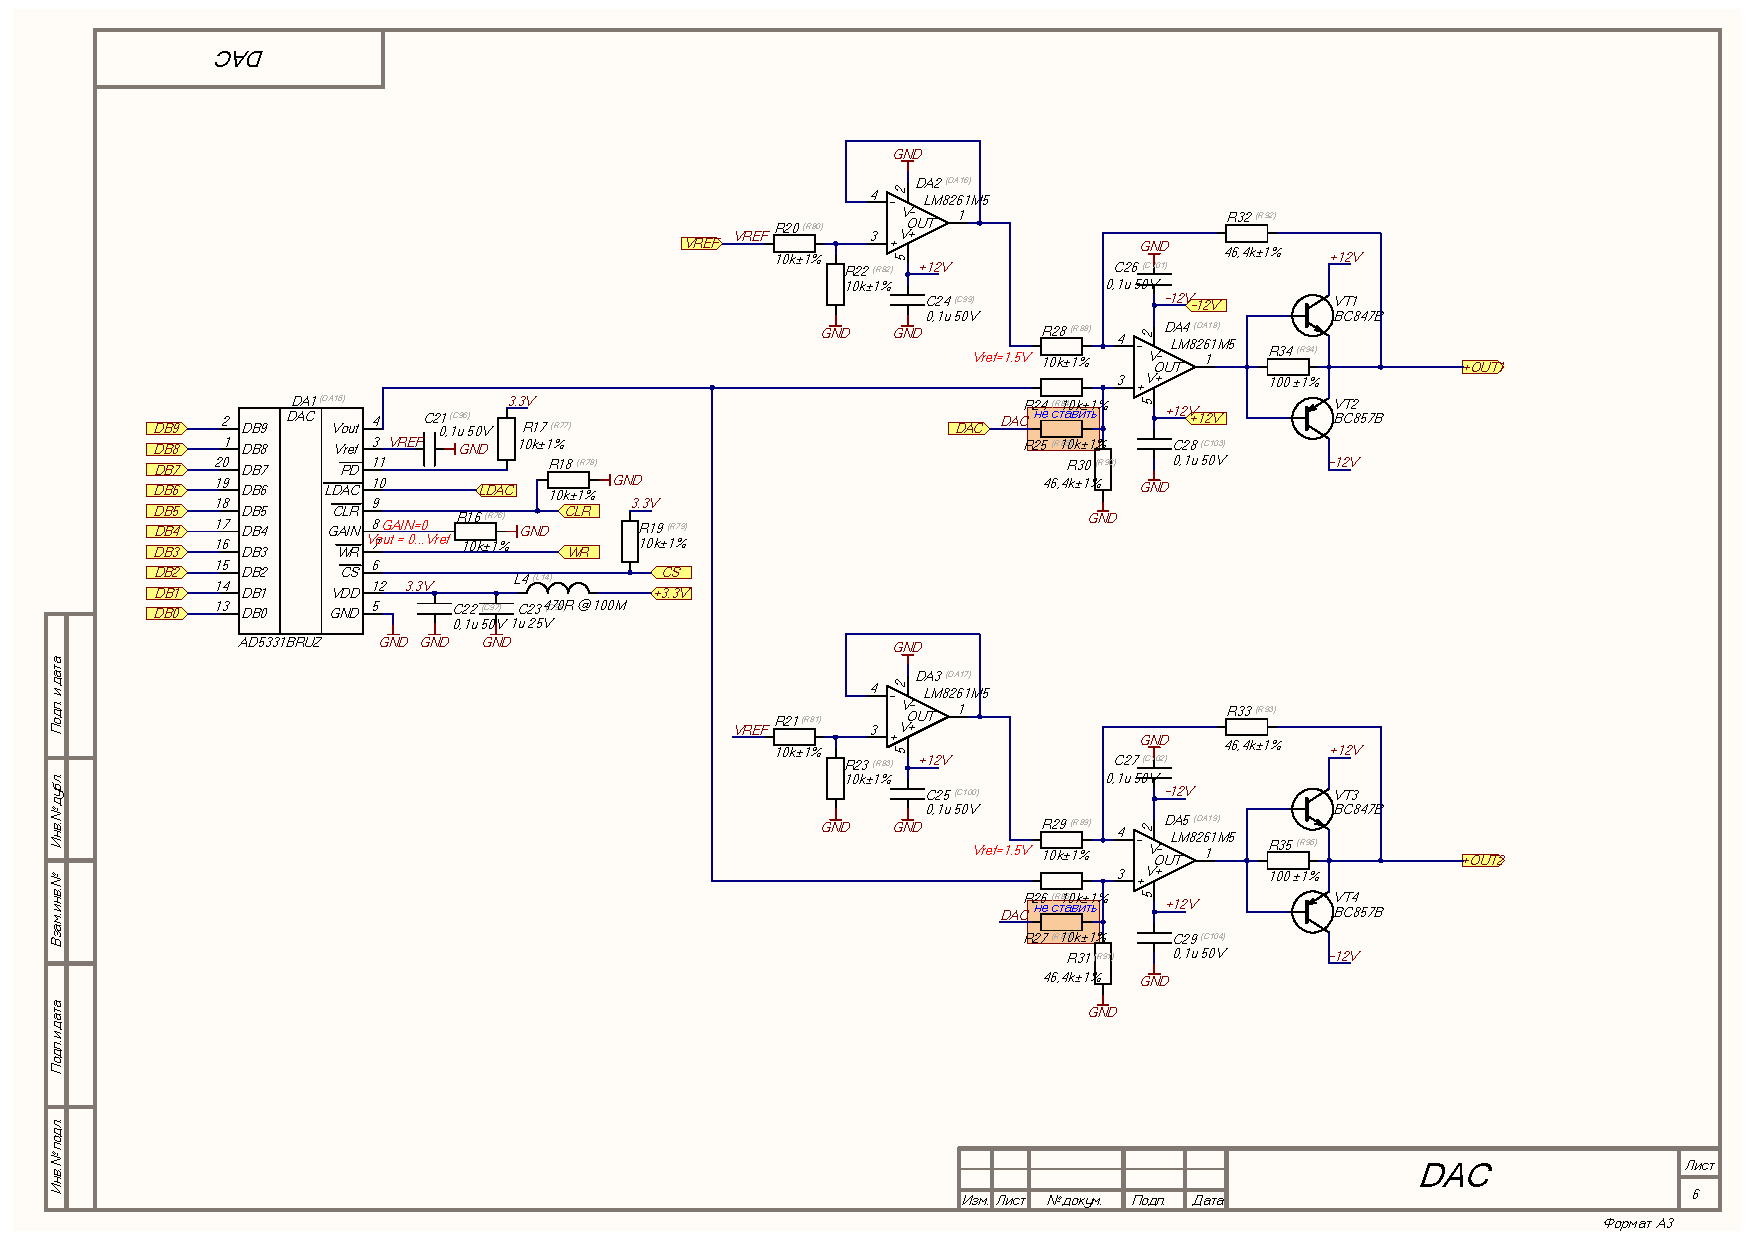
\includepdf[pages=1, scale=0.75, angle=-90, pagecommand={}]{DAC.pdf}

%     \caption{Схема включения ЦАП} \label{DAC}
% \end{figure}

% \begin{figure}[h!]
%     \centering
%     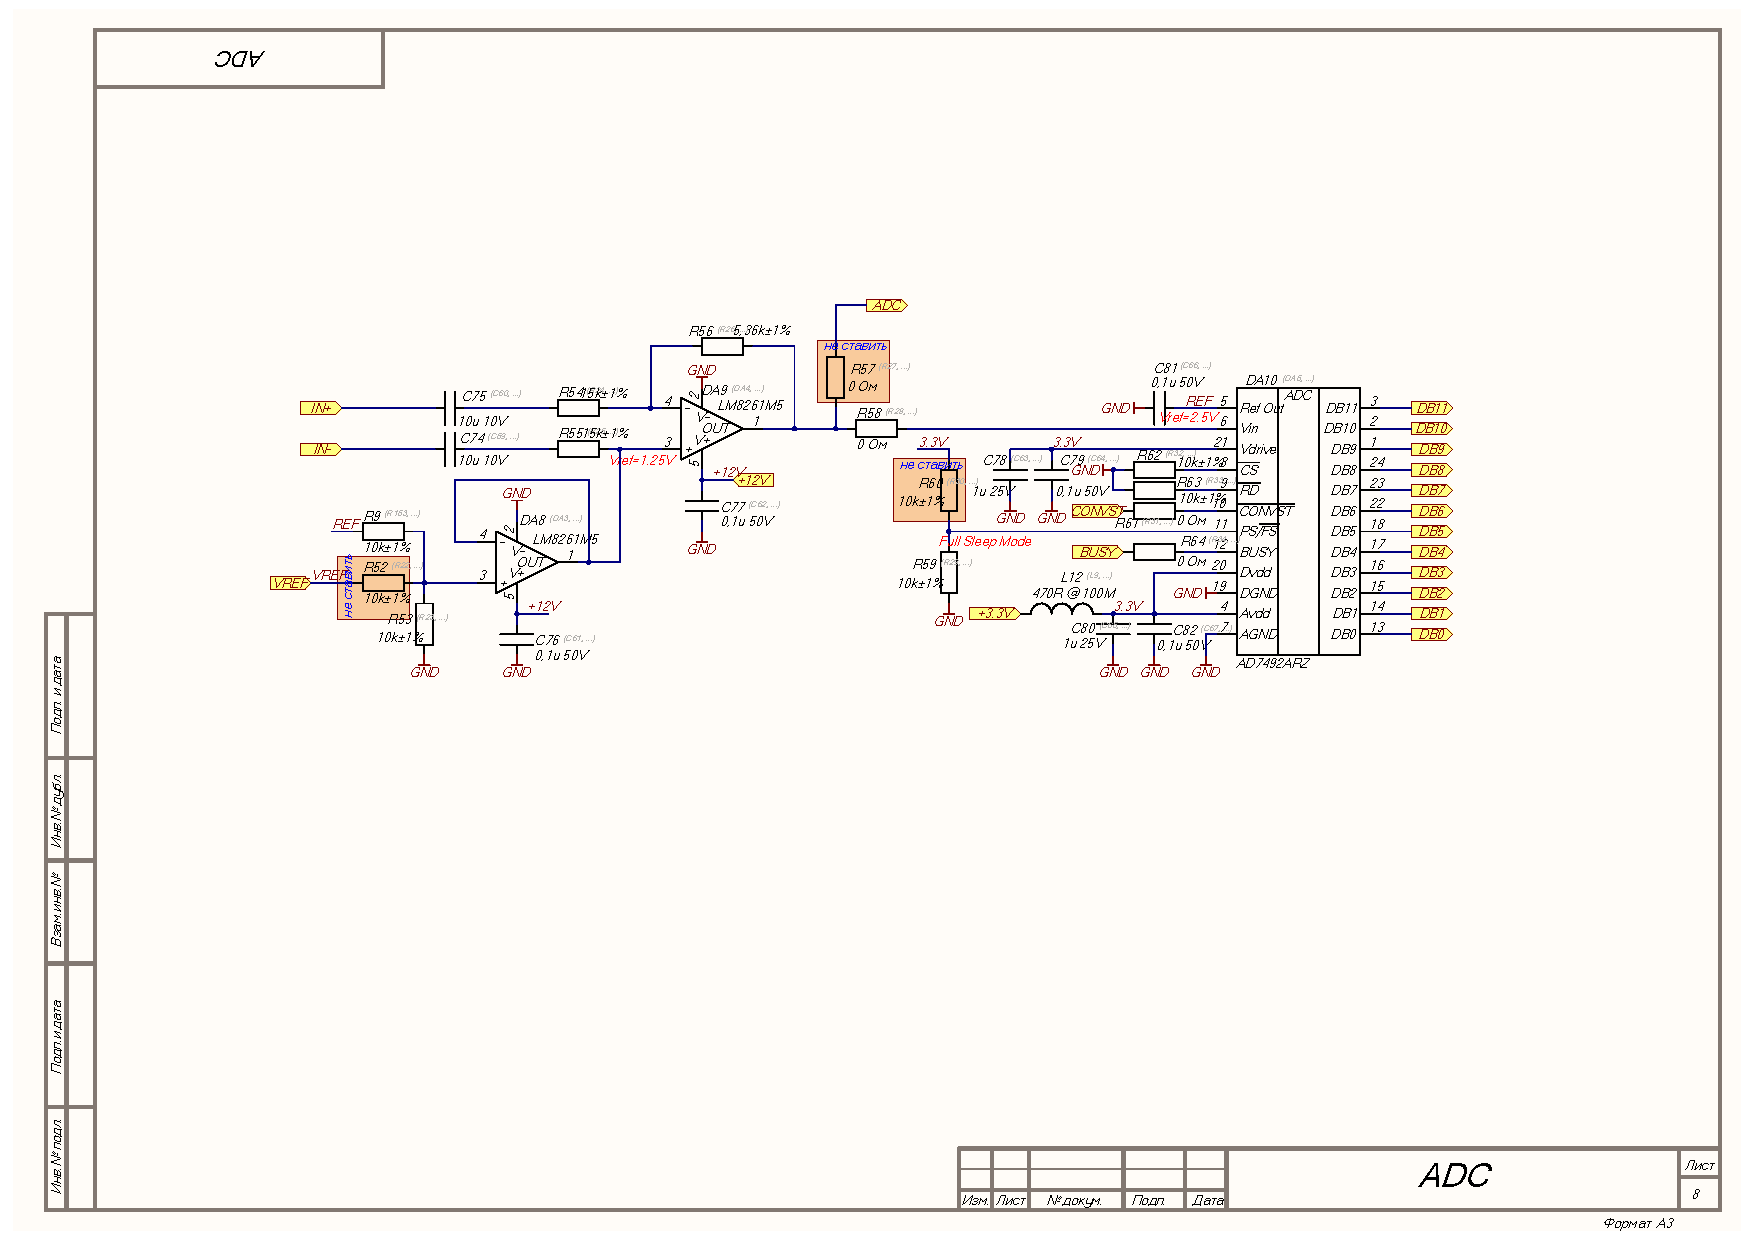
\includepdf[pages=1, scale=0.75, angle=-90, pagecommand={}]{ADC.pdf}

%     \caption{Схема включения АЦП} \label{ADC}
% \end{figure}
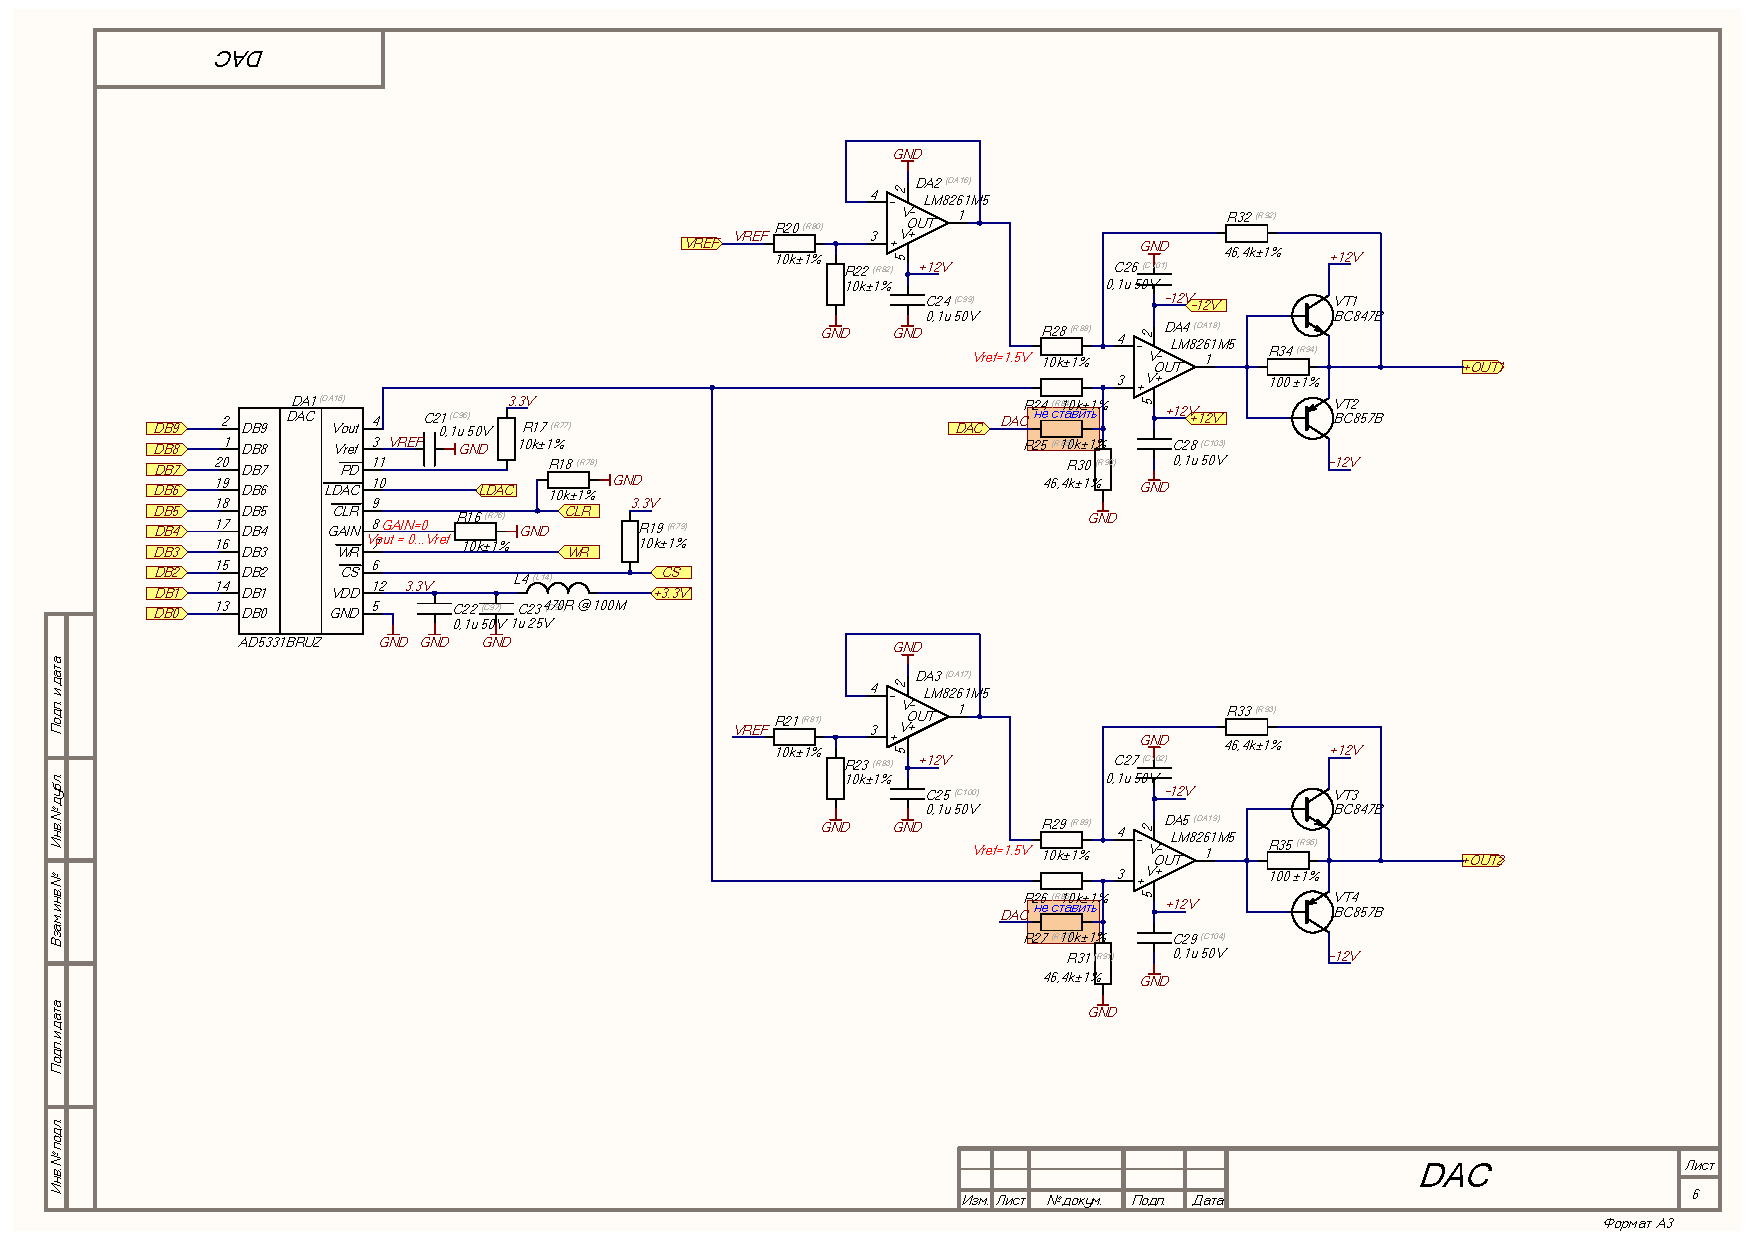
\includepdf[pages=1, scale=0.8, angle=90, pagecommand=\label{DAC}]{DAC.pdf}
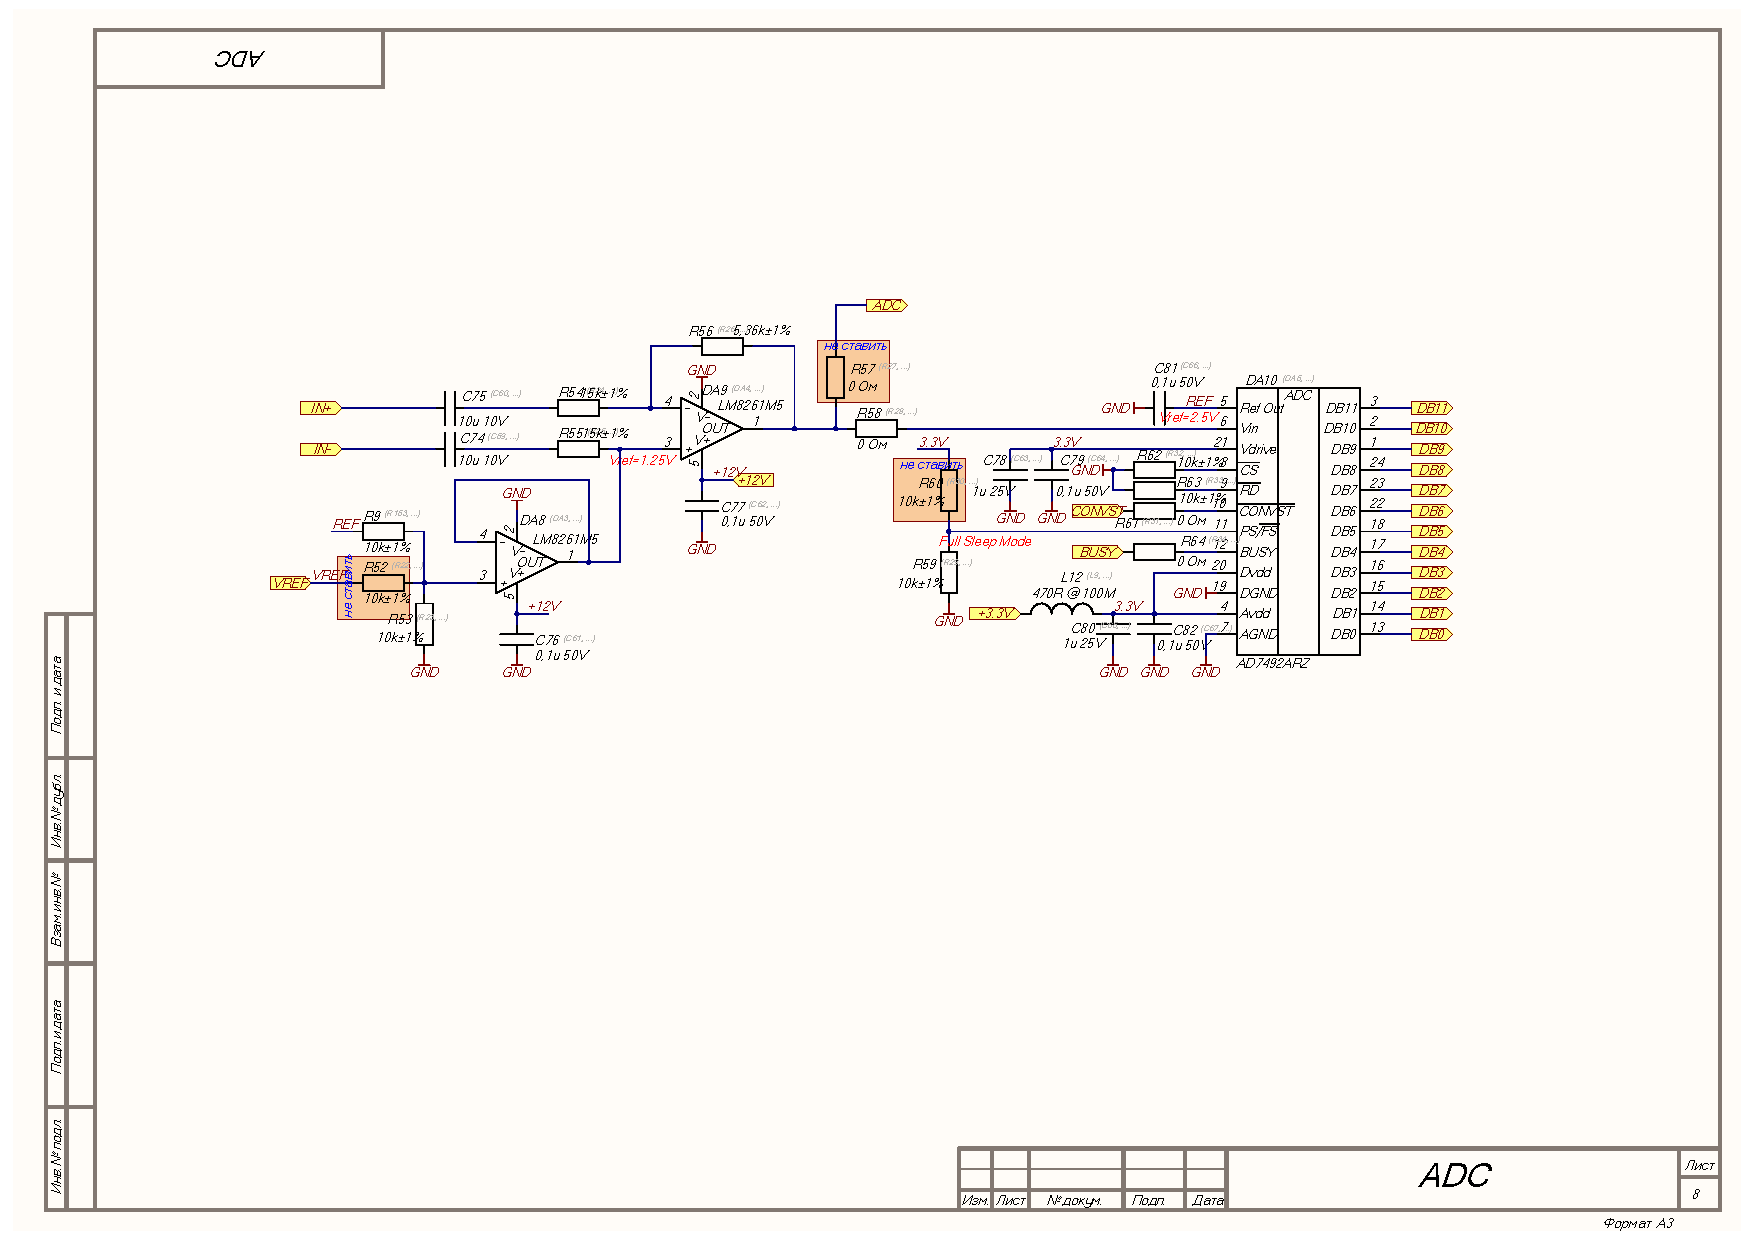
\includepdf[pages=1, scale=0.8, angle=90, pagecommand=\label{ADC}]{ADC.pdf}
\clearpage
% \restoregeometry